%
% kontur-allgemein.tex
%
% (c) 2026 Damien Flury, OST Ostschweizer Fachhochschule
%
\begin{figure}
\centering
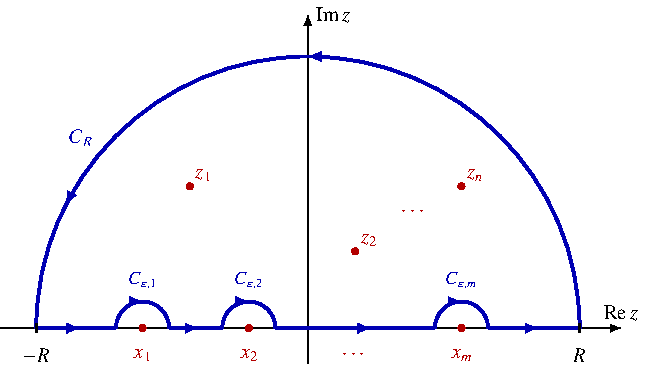
\includegraphics{papers/hauptwert/images/kontur-allgemein.pdf}
\caption{Der Integrationsweg $\Gamma$ im Beweis von
Satz~\ref{hauptwert:satz:hauptformel}, im positiven Sinn durchlaufen.
Auf der reellen Achse wird von $-R$ bis $R$ integriert, wobei um jede
Polstelle $x_j$ das Intervall $[x_j-\varepsilon, x_j+\varepsilon]$
ausgespart und durch die Einbuchtung $C_{\varepsilon,j}$ ersetzt wird.
Der grosse Halbkreis $C_R$ schliesst den Weg.
Die Einbuchtungen halten die Polstellen $x_1,\dots,x_m$ ausserhalb des
umlaufenen Gebietes, innerhalb liegen daher genau die Polstellen
$z_1,\dots,z_n$ der oberen Halbebene.
\label{hauptwert:figure:kontur-allgemein}}
\end{figure}
